\begin{figure*}
\begin{tikzpicture}[
squaredred/.style={rectangle, draw=black!60, fill=red!5, very thick, minimum size=5mm},
squaredblue/.style={rectangle, draw=black!60, fill=blue!5, very thick,minimum size=5mm},
squaredgreen/.style={rectangle, draw=black!60, fill=green!5, very thick, minimum size=5mm},
]
%Nodes
\node[squaredred] (articlepic)
{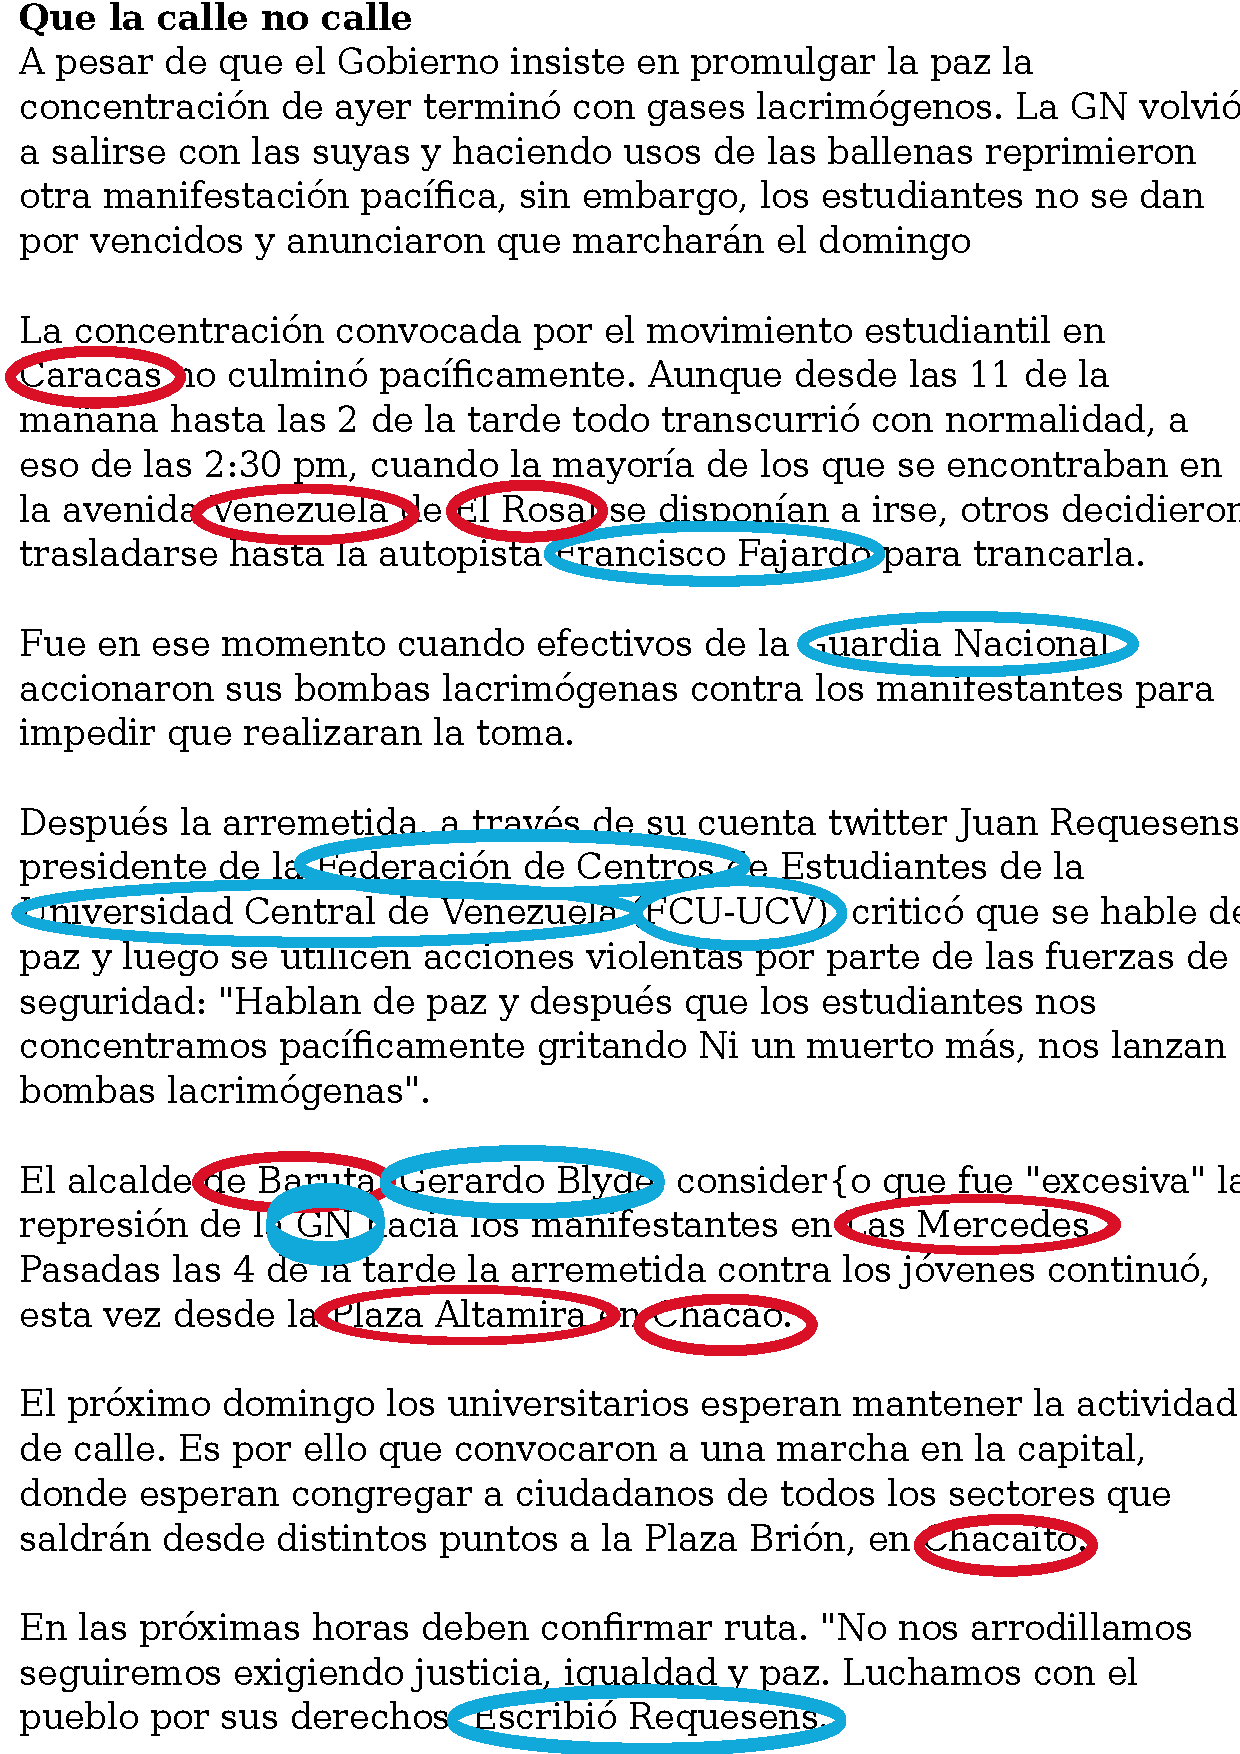
\includegraphics[height=0.25\textheight]{figures/article}};

\node[squaredblue](geodist) [right=of articlepic,
align=center,scale=0.68]
{\{"Admin1":"Caracas",\\
"city": "Caracas",\\
"country": "Caracas",\\
"confidence": 0.4218\}
\\
\\
\{"Admin1": "Miranda",\\
"city": "Baruta",\\
"country": "Venezuela",\\
"confidence": 0.2639\},
\\
\\
\{"Admin1": "Miranda",\\
"city": "Chacao",\\
"country": "Venezuela",\\
"confidence": 0.2639\},
%\\
\\
\{"Admin1": "Ciego de Avila",\\
"city": "Venezuela",\\
"country": "Cuba",\\
"confidence": "0.0511"\},
%\\
\\
\{"Admin1": "Cundinamarca",\\
"city": "El Rosal",\\
"country": "Colombia",\\
"confidence": 0.0012\},
};


\node[squaredgreen] (finalgeo) [right=of geodist, align=left, scale=0.7] {Admin1: Caracas,\\
                                                 City: Caracas,\\
                                                 Country: Venezuela\\
                                                 Confidence: 0.4218};
%Lines
\draw[very thick, ->] (articlepic.east) -- (geodist.west);
\draw[very thick, ->] (geodist.east) -- (finalgeo.west);

\end{tikzpicture}
\caption{An example of location inference using PSL. Red circles
   denote named entities identified as locations and blue denotes other
   types of entities. The article describes students planning a march on
   Sunday.  It identifies multiple locations, e.g., Chacao, El Roso, and
   the Francisco Fajardo highway where protests have been happening.
   There is also a reference to a quote by the mayor of Baruto.
   Mentions of such multiple locations are resolved using our PSL
   program to the intended location, here Caracas.}
\label{fig:psl_example}

\end{figure*}
